\section{From automaton to regular expression}

Consider a scenario where, for simplicity, the initial state $i$ is unique, having no incoming arcs, and similarly, the final state $t$ is unique without outgoing arcs.
Any state other than $i$ and $t$ is referred to as internal.
To establish an equivalent automaton, denoted as a generalized finite automaton, we extend the capability of arc labels to encompass regular languages.

The process involves eliminating internal nodes one by one.
After each elimination, one or more compensation arcs are added to maintain the equivalence of the automaton. 
These new arcs are labeled by regular expressions.
Eventually, only the nodes $i$ and $t$ remain, connected by a single arc from $i$ to $t$. 
The regular expression labeling this arc generates the complete language recognized by the original finite automaton.

The order in which eliminations are performed is not crucial. 
However, different orders may yield distinct regular expressions, all equivalent to each other but varying in complexity.
\begin{example}
    Consider the given automaton:
    \begin{figure}[H]
        \centering
        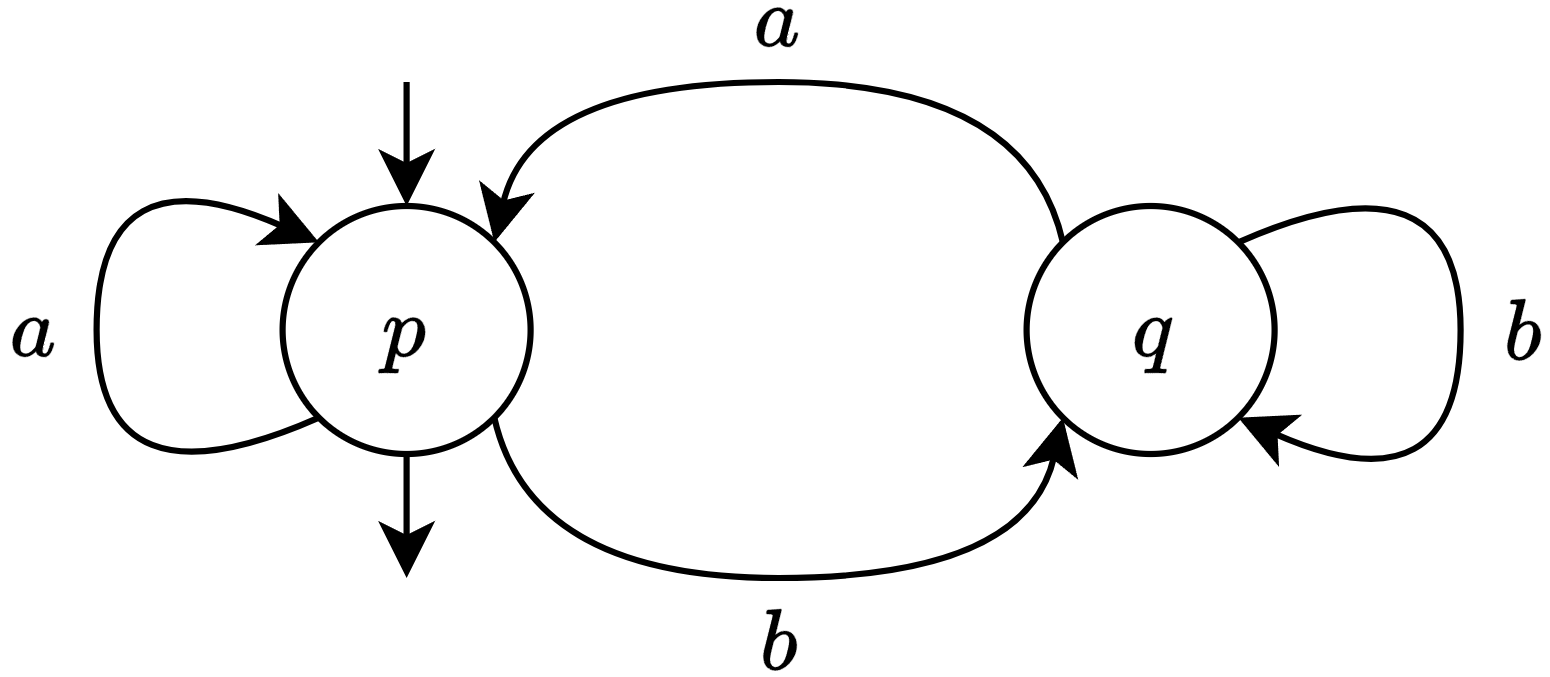
\includegraphics[width=0.35\linewidth]{images/br1.png}
    \end{figure}
    To normalize it and designate the initial and final states, we obtain:
    \begin{figure}[H]
        \centering
        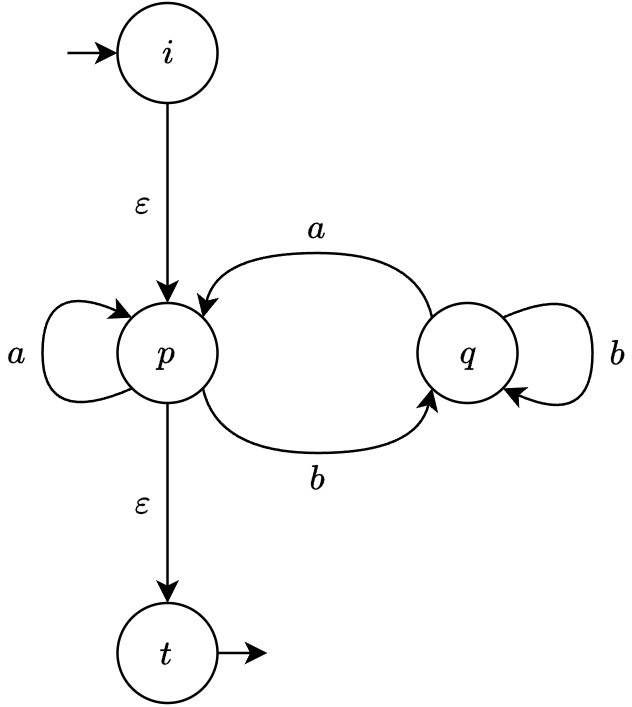
\includegraphics[width=0.35\linewidth]{images/br2.png}
    \end{figure}
    Finally, we apply the Brzozowski and McCluskey method to the normalized automaton in three steps:
    \begin{enumerate}
        \item Eliminate the node $q$, replacing it with the regular expression $bb^{\ast}a$.
        \item Merge the two cycles on node $p$ with the choice operator, resulting in $a\mid bb^{\ast}a=b^{\ast}a$. 
        \item Remove the node $p$ by replacing the label of the arc with $(b^{\ast}a)^{\ast}$. 
    \end{enumerate}
    The resulting automaton after these steps is as follows:
    \begin{figure}[H]
        \centering
        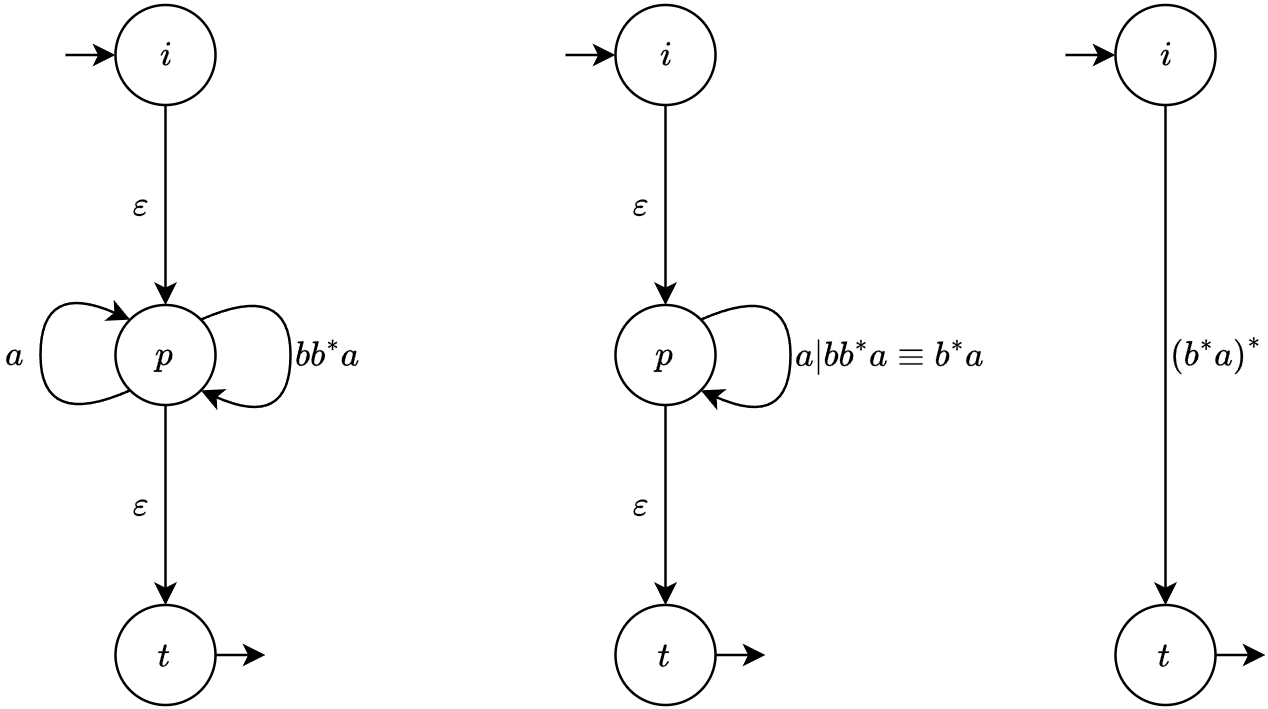
\includegraphics[width=0.65\linewidth]{images/br3.png}
    \end{figure}
\end{example}